\title{The Cauchy basis}

In this note we describe the construction of the {\bf Cauchy basis}, whose
functions satisfy at the same time Dirichlet and Neumann boundary conditions.
Besides being beautiful, it is useful to solve fourth-order boundary
problems.


\section{Introduction: Fourier, cosine and sine basis}

Everybody knows the Fourier basis of $L^2([0,2\pi])$, defined by sine and
cosine functions of integer frequencies.

$$
	1,\cos(x),\cos(2x),\ldots,\sin(x),\sin(2x),\ldots
$$

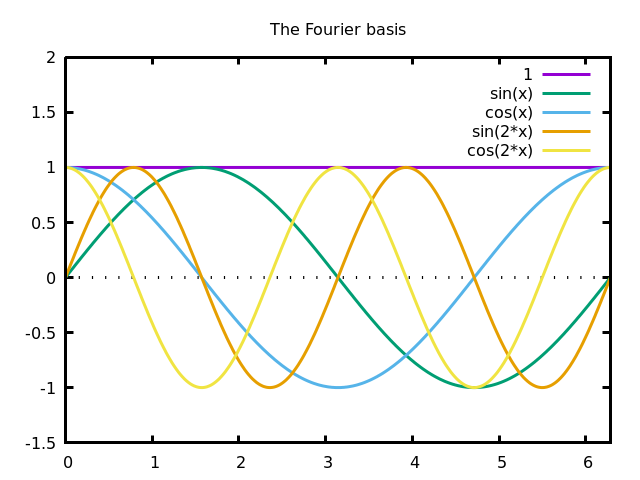
\includegraphics{sincos.png}
%SCRIPT gnuplot <<END >sincos.png
%SCRIPT set term pngcairo lw 3
%SCRIPT set title "The Fourier basis"
%SCRIPT set samples 1000
%SCRIPT set zeroaxis
%SCRIPT plot [0:2*pi] [-1.5:2] 1,sin(x),cos(x),sin(2*x),cos(2*x)
%SCRIPT END


This was the original basis used by Joseph Fourier to study the heat equation.
Notice that cosines are symmetric around the center of the interval, and
sines are anti-symmetric.  Thus, all the functions of this basis are
necessary to represent arbitrary functions on the whole interval.

Less well-known are the cosine basis, defined by cosines of half-integer
frequencies
$$
1,\cos\left(\frac{1}{2}x\right),
\cos(x),
\cos\left(\frac{3}{2}x\right),
\cos(2x),\ldots
$$

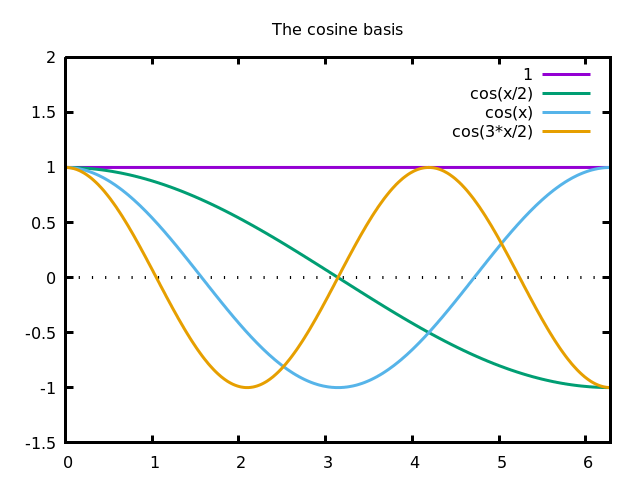
\includegraphics{cos.png}
%SCRIPT gnuplot <<END >cos.png
%SCRIPT set term pngcairo lw 3
%SCRIPT set title "The cosine basis"
%SCRIPT set samples 1000
%SCRIPT set zeroaxis
%SCRIPT plot [0:2*pi] [-1.5:2] 1,cos(x/2),cos(x),cos(3*x/2)
%SCRIPT END


and the sine basis, defined by sines of half-integer frequencies
$$
\sin\left(\frac{1}{2}x\right),
\sin(x),
\sin\left(\frac{3}{2}x\right),
\sin(2x), \ldots
$$

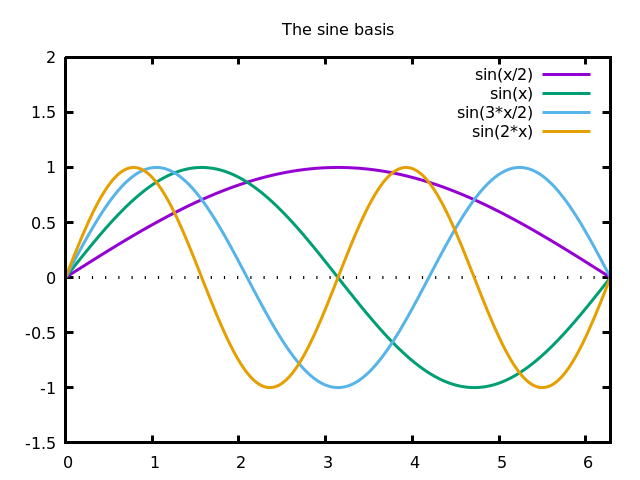
\includegraphics{sin.png}
%SCRIPT gnuplot <<END >sin.png
%SCRIPT set term pngcairo lw 3
%SCRIPT set title "The sine basis"
%SCRIPT set samples 1000
%SCRIPT set zeroaxis
%SCRIPT plot [0:2*pi] [-1.5:2] sin(x/2),sin(x),sin(3*x/2),sin(2*x)
%SCRIPT END


Each one of these three sequences of functions is a Hilbert basis of the
space~$L^2([0,2\pi])$.  In particular, you can express a sine as a linear
combination of cosines, and vice-versa.  This is a favourite exam question of
mine.  Of course, the convergence is not uniform on the boundaries of the
interval.

The cosine and sine bases are very useful when you want to express solutions of
a differential equation (or a variational problem) satisfying particular
boundary conditions.  Notice that if~$f(x)$ is a finite linear combination of
the sine basis, then~$f(0)=f(2\pi)=0$ and if it is a finite linear combination
of the cosine basis, then~$f'(0)=f'(2\pi)=0$.  The same relationships hold for
series as long as the coefficients decrease fast enough.  Thus, the sine basis
is useful for \emph{Dirichlet boundary conditions}, and the cosine basis is
useful for \emph{Neumann boundary conditions}.


\section{The Cauchy basis}

The functions of the Cauchy basis, defined below, satisfy simultaneously the
four conditions~$f(0)=f(1)=f'(0)=f'(1)=0$.

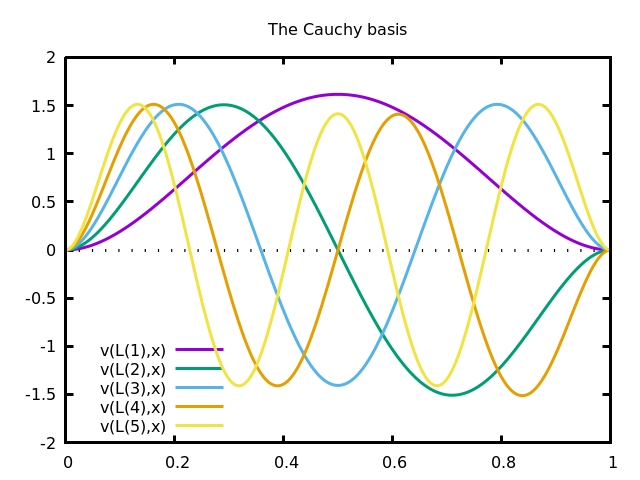
\includegraphics{cauchy.png}
%SCRIPT gnuplot <<END >cauchy.png
%SCRIPT set term pngcairo lw 3
%SCRIPT set title "The Cauchy basis"
%SCRIPT # define eigenvalues (good enough approximation)
%SCRIPT L(n) = (2*n+1)*pi/2-(-1)**n*2*exp(-(2*n+1)*pi/2)
%SCRIPT
%SCRIPT # define eigenvectors
%SCRIPT b(l) = (sinh(l)-sin(l))/(cos(l)-cosh(l))
%SCRIPT v(l,x) = sin(l*x)-sinh(l*x)+b(l)*(cos(l*x)-cosh(l*x))
%SCRIPT
%SCRIPT # plot the first few functions
%SCRIPT set key bottom left
%SCRIPT set samples 1000
%SCRIPT set zeroaxis
%SCRIPT plot [-0:1] [-2:2] v(L(1),x),v(L(2),x),v(L(3),x),v(L(4),x),v(L(5),x)
%SCRIPT END


A simple construction of such a set of functions is obtained by considering
eigenfunctions of the fourth derivative that satisfy the four boundary
conditions.

Eigenfunctions of the fourth derivative are of the form~$\exp(\rho x)$
where~$\rho$ is a fourth-root of~$1$, thus $\rho\in\{1,-1,i,-i\}$.
Equivalently, they are linear combinations of~$\sin$, $\cos$, $\sinh$ and
$\cosh$

$$
\varphi(x)=\alpha\cos(\lambda x)+\beta\sin(\lambda x)+\gamma\cosh(\lambda
x)+\delta\sinh(\lambda x)
$$

This is an eigenfunction of the fourth derivative with
eigenvalue~$\lambda^4$, that we can assume to be real positive.

By imposing the four boundary conditions, we obtain a linear system on the
coefficients~$(\alpha,\beta,\gamma,\delta)$, with a parameter~$\lambda$.  The
matrix of this linear system is singular, and its determinant vanishes
when~$\lambda$ satisfies the equation
$$
\cos\lambda\cosh\lambda=1
$$
The solutions of this equation (which are slight perturbations of even
multiples of~$pi/2$)
are the eigenvalues of our basis.

A good enough approximation is given by
$$
\lambda_n = \frac{2n+1}{2}\pi - (-1)^n2\exp\left(-\frac{(2n+1)}{2}\pi\right)
$$
and the eigenfunctions are thus
$$
\varphi_n(x)=\sin(\lambda_nx)-\sinh(\lambda_nx)+\beta_n(\cos(\lambda_nx)-\cosh(\lambda_nx))
$$
where
$$
\beta_n=\frac{\sinh\lambda_n-\sin\lambda_n}{\cos\lambda_n-\cosh\lambda_n}.
$$

Notice that, although the functions~$\varphi_n$ are beautiful and symmetric
inside the interval~$[0,1]$, they explode in wild ways outside this interval:

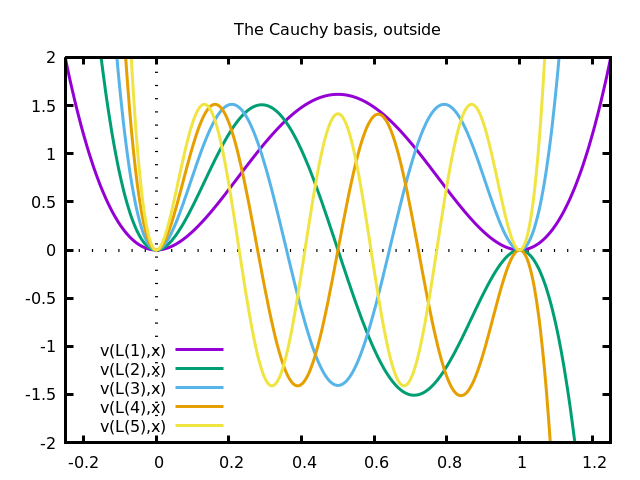
\includegraphics{cauchy2.png}
%SCRIPT gnuplot <<END >cauchy2.png
%SCRIPT set term pngcairo lw 3
%SCRIPT set title "The Cauchy basis, outside"
%SCRIPT set samples 1000
%SCRIPT # define eigenvalues (good enough approximation)
%SCRIPT L(n)=(2*n+1)*pi/2-(-1)**n*2*exp(-(2*n+1)*pi/2)
%SCRIPT
%SCRIPT # define eigenvectors
%SCRIPT b(l)=(sinh(l)-sin(l))/(cos(l)-cosh(l))
%SCRIPT v(l,x)=sin(l*x)-sinh(l*x)+b(l)*(cos(l*x)-cosh(l*x))
%SCRIPT
%SCRIPT # plot the first few functions
%SCRIPT set key bottom left
%SCRIPT set samples 1000
%SCRIPT set zeroaxis
%SCRIPT plot [-0.25:1.25] [-2:2] v(L(1),x),v(L(2),x),v(L(3),x),v(L(4),x),v(L(5),x)
%SCRIPT END

\section{Properties and open problems}

We have just defined a set of functions~$\varphi_n(x)$.  By construction,
they are $C^\infty$ functions on the interval~$[0,1]$ that
satisfy~$0=\varphi_n(0)=\varphi_n(1)=\varphi_n'(0)=\varphi_n'(1)$.  Since
these functions are eigenvectors of a linear operator with different
eigenvalues, they must be orthogonal.  The following remains to be
done:

\begin{enumerate}
	\item Prove that $\{\varphi_n(x)\}$ is a Hilbert basis of $L^2([0,1])$
	\item Prove that $|\varphi_n(x)|\le 2$ for~$x\in[0,1]$
	\item Prove that $\varphi_{2n}(x)=-\varphi_{2n}(1-x)$ for~$x\in[0,1]$
		(so that~$\varphi_{2n}(1/2)=0$).
	\item Prove that $\varphi_{2n+1}(x)=\varphi_{2n+1}(1-x)$ for~$x\in[0,1]$
		(so that~$\varphi'_{2n+1}(1/2)=0$).
	\item Prove that~$\varphi_n$ has~$n-1$ zeros on~$(0,1)$, and identify
		them.
	\item Compute the exact normalization coefficients required so that the
		basis is orthonormal.
	\item Obtain an effective algorithm/formula to evaluate
		~$\varphi_n(x)$ for large values of~$n$, avoiding the
		numerical cancellations that appear with the current
		expression.  Notice that, thanks to the symmetry properties
		above, the formula only needs to be stable for~$0\le
		x\le\frac{1}{2}$ (the difficult case being
		near~$\frac{1}{2}$).
	\item Rewrite the definition so that the interval is centered around
		0, and the symmetries are more visible.
	\item Study how the regularity of a function can be measured from the
		rate of decrease of its "Cauchy coefficients"
	\item Develop a theory of sampling using "Cauchy polynomials" as an
		interpolation model
	\item Develop a "Fast Cauchy Transform", to obtain the coefficients
		of these polynomials from their samples.
	\item Extend this basis to the case of a square.
	\item Extend this basis to the case of a disk.
\end{enumerate}

Some of these propositions are easy, others may not actually be possible
(especially the last one).

\section{Detailed calculation}

In this section we detail the construction leading to the Cauchy basis.
The computation has two parts.  First, we explain how the
equation~$\cos\lambda\cosh\lambda=1$ is obtained,
and then we propose a numerical approximation of the solutions of this
equation.


\subsection{The eigenvalue equation}
We start with the basic form
$$
\varphi(x)=
\alpha\cos\lambda x
+\beta\sin\lambda x
+\gamma\cosh\lambda x
+\delta\sinh\lambda x
$$
and we want to determine values of the five
parameters~$\alpha,\beta,\gamma,\delta,\lambda$ so that~$\varphi$ satisfies
the four boundary conditions~$0=\varphi(0)=\varphi(1)=\varphi'(0)=\varphi'(1)$.
We have
$$
\varphi'(x)=\lambda\left[
	-\alpha\sin\lambda x
	+\beta\cos\lambda x
	+\gamma\sinh\lambda x
	+\delta\cosh\lambda x
\right]
$$
And setting~$0=\varphi(0)$ and~$0=\varphi'(0)$ gives
respectively~$\gamma=-\alpha$ and~$\delta=-\beta$, thus
$$
\varphi(x)=
	\alpha\left(\cos\lambda x-\cosh\lambda x\right)
	+
	\beta\left(\sin\lambda x-\sinh\lambda x\right)
$$
and
$$
\varphi'(x)=\lambda
\left[
	\alpha\left(-\sin\lambda x-\sinh\lambda x\right)
	+
	\beta\left(\cos\lambda x-\cosh\lambda x\right)
	\right]
$$
To simplify the notation, we write
\begin{eqnarray*}
	c &= \cos\lambda \\
	s &= \sin\lambda \\
	k &= \cosh\lambda \\
	z &= \sinh\lambda \\
\end{eqnarray*}
thus the conditions~$0=\varphi(1)$ and~$0=\varphi'(1)$ read
\begin{eqnarray*}
	0 &= \alpha(c-k)+\beta(s-z) \\
	0 &= \alpha(-s-z)+\beta(c-k) \\
\end{eqnarray*}
or, in matrix form
$$
\begin{pmatrix}
	c-k & s-z \\
	-s-z & c-k \\
\end{pmatrix}
\begin{pmatrix}
	\alpha \\
	\beta \\
\end{pmatrix}
=
\begin{pmatrix}
	0 \\
	0 \\
\end{pmatrix}
$$
If~$(\alpha,\beta)$ is not the zero vector, then the matrix must be singular,
thus
$$
(c-k)^2+(s+z)(s-z)=0
$$
this condition can be simplified using the trigonometric
identities~$c^2+s^2=1$ and~$k^2-z^2=1$ to obtain the equivalent
equation~$ck=1$ :
$$
\cos\lambda\cosh\lambda=1
$$
Besides the non-interesting case~$\lambda=0$, this equation has an infinite
sequence of solutions~$\pm\lambda_n$ that determine the spectrum of our
problem.  Given such a solution~$\lambda_n$, the corresponding values
of~$\alpha_n,\beta_n$ are determined from the condition~$0=\varphi(1)$:
$$
0 =
\alpha_n(\cos\lambda_n-\cosh\lambda_n)
+\beta_n(\sin\lambda_n-\sinh\lambda_n)
$$
we normalize the solution with~$\alpha_n=1$ (this is an arbitrary choice,
maybe not the best one, but it produces nicely bounded functions on~$[0,1]$).  Now
$$
\beta_n=\frac{\cos\lambda_n-\cosh\lambda_n}{\sinh\lambda_n-\sin\lambda_n}
$$
and the functions of the basis are
$$
\varphi_n(x)=\sin(\lambda_nx)-\sinh(\lambda_nx)+\beta_n(\cos(\lambda_nx)-\cosh(\lambda_nx))
$$
Or, by rearranging the terms,
$$
\varphi_n(x)=
\frac{
 (\beta_n-1) e^{\lambda_nx}
+(\beta_n+1) e^{-\lambda_nx}
+(\beta_n-i) e^{i\lambda_nx}
+(\beta_n+i) e^{-i\lambda_nx}
}{2}
$$
or even
$$
\varphi_n(x)=\frac{1}{2}\sum_{\rho^4=1}
(\beta_n-\rho)e^{\rho\lambda_n x}
$$
and this last expression is more amenable to computations (derivatives,
integrals, scalar products).

\subsection{Numerical solution of the eigenvalue equation}

By plotting the function~$x\to\cos x\cosh x$, it is clear that it crosses the
value~$1$ infinitely many times, very near to the zeros of~$\cos x$, except
for~$x=\pi/2$:

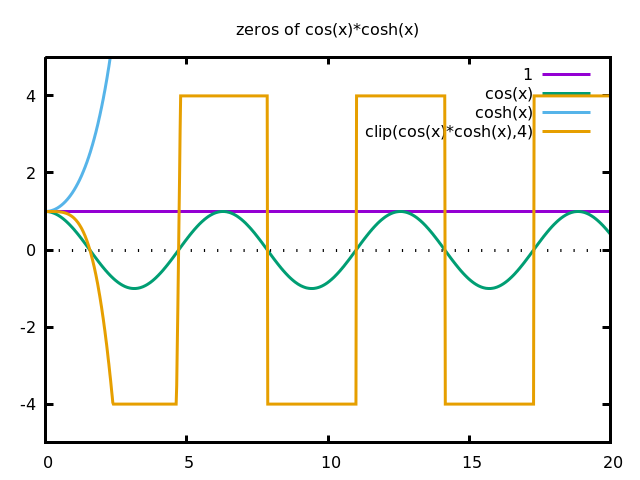
\includegraphics{coscosh.png}
%SCRIPT gnuplot <<END >coscosh.png
%SCRIPT set term pngcairo lw 3
%SCRIPT set title "zeros of cos(x)*cosh(x)"
%SCRIPT
%SCRIPT fmax(a,b)=a<b?b:a
%SCRIPT fmin(a,b)=a<b?a:b
%SCRIPT clip(x,a)=fmax(fmin(x,a),-a)
%SCRIPT
%SCRIPT set samples 1000
%SCRIPT set zeroaxis
%SCRIPT plot [0:20] [-5:5] 1,cos(x),cosh(x),clip(cos(x)*cosh(x),4)
%SCRIPT END


Thus, the zeros of the function~$\lambda\to\cos\lambda\cosh\lambda-1$ have the
form
$$
\lambda_n = \frac{2n+1}{2}\pi + \varepsilon_n
$$
where~$\varepsilon_n$ are numbers that tend very fast to zero and alternate
sign.
We can estimate the number~$\varepsilon_n$ by computing the tangent to the
graph of~$\cos x\cosh x$ at~$x=\frac{2n+1}{2}\pi$, and finding its
intersection with the horizontal line~$y=1$:
$$
1 = \cos x_n\cosh x_n +
\left(
\cos x_n\sinh x_n - \sin x_n\cosh x_n
\right) \varepsilon_n
$$
for $x_n=\frac{2n+1}{2}\pi$.  Since~$\cos x_n=0$ and~$\sin x_n=-(-1)^n$, this
simplifies to
$$
\varepsilon_n=\frac{-(-1)^n}{\cosh x_n} \approx -2e^{-x_n}
$$
resulting in the approximation proposed above
$$
\lambda_n\approx\frac{2n+1}{2}\pi-2(-1)^n\exp\left(-\frac{2n+1}{2}\pi\right).
$$
This approximation is useful, at least for plotting purposes.
Notice that the quality of the approximation improves as~$n$ grows, so a
satisfactory solution can be attained by tabulating the exact values
of~$\lambda_n$ for small values of~$n$, and using the approximation for the
others.




\section{Computer code}
This is the complete \verb+gnuplot+ code to produce plots of the Cauchy
basis:

\begin{verbatim}
X(n)   = (2*n+1)*pi/2                 # approximate eigenvalues (to 0th order)
L(n)   = X(n) - (-1)**n/cosh(X(n))    # refined eigenvalues (to 1st order)
s(x)   = sin(x) - sinh(x)             # notation
c(x)   = cos(x) - cosh(x)             # notation
u(l,x) = s(l*x) - c(l*x) * s(l)/c(l)  # generic eigenfunction
v(n,x) = u(L(n),x)                    # n-th eigenfunction
plot [-0:1] [-2:3] v(1,x),v(2,x),v(3,x),v(4,x),v(5,x)
\end{verbatim}

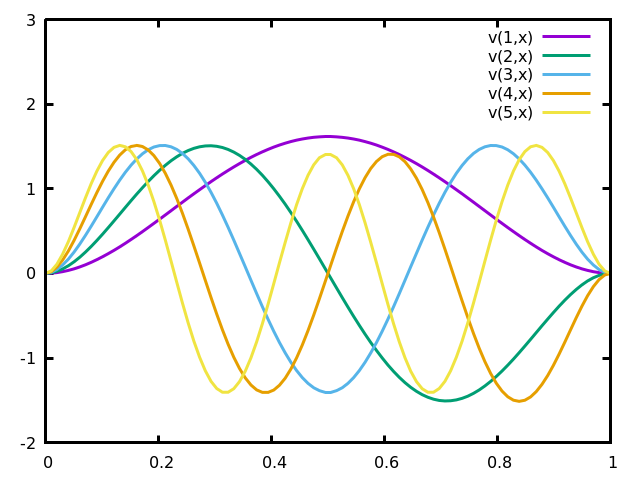
\includegraphics{cauchy3.png}
%SCRIPT gnuplot <<END >cauchy3.png
%SCRIPT set term pngcairo lw 3
%SCRIPT X(n) = (2*n+1)*pi/2
%SCRIPT L(n) = X(n) - (-1)**n/cosh(X(n))
%SCRIPT s(x) = sin(x) - sinh(x)
%SCRIPT c(x) = cos(x) - cosh(x)
%SCRIPT u(l,x) = s(l*x) - c(l*x) * s(l)/c(l)
%SCRIPT v(n,x) = u(L(n),x)
%SCRIPT plot [-0:1] [-2:3] v(1,x),v(2,x),v(3,x),v(4,x),v(5,x)
%SCRIPT END





% vim:set tw=77 filetype=tex spell spelllang=en:
